Ausgecheckt und den beim ersten Hafenrundgang entdeckten Flugzeugträger USS Midway angefahren.
Vor Ort haben wir ein Parkuhrticket für $1 \frac{1}{2}$ Stunden gelöst, weil ich der Über\-zeugung war, dass das Ding bestimmt nicht mehr hergibt.
Denkste.
Auf dem Flugdeck alleine steht genug Material in Form von Hubschraubern und Kampfjets für eine gute Stunde herum.
Unter Deck sind wir durch die Schlafkabinen der Mannschafter und Offiziere sowie den \FOREIGN{Ready Room}\footnote{Einsatzbesprechungsraum} spaziert.
Sämtliche Abzweigungsmöglichkeiten sind ab- bzw. versperrt, in dem Labyrinth soll sich schließlich niemand verlaufen.
Unter Deck 

%\newpage
%\thispagestyle{empty}
\begin{tikzpicture}[remember picture, overlay]
\node[inner sep=0pt, yshift=-.2\paperheight] at (current page.north) {%
	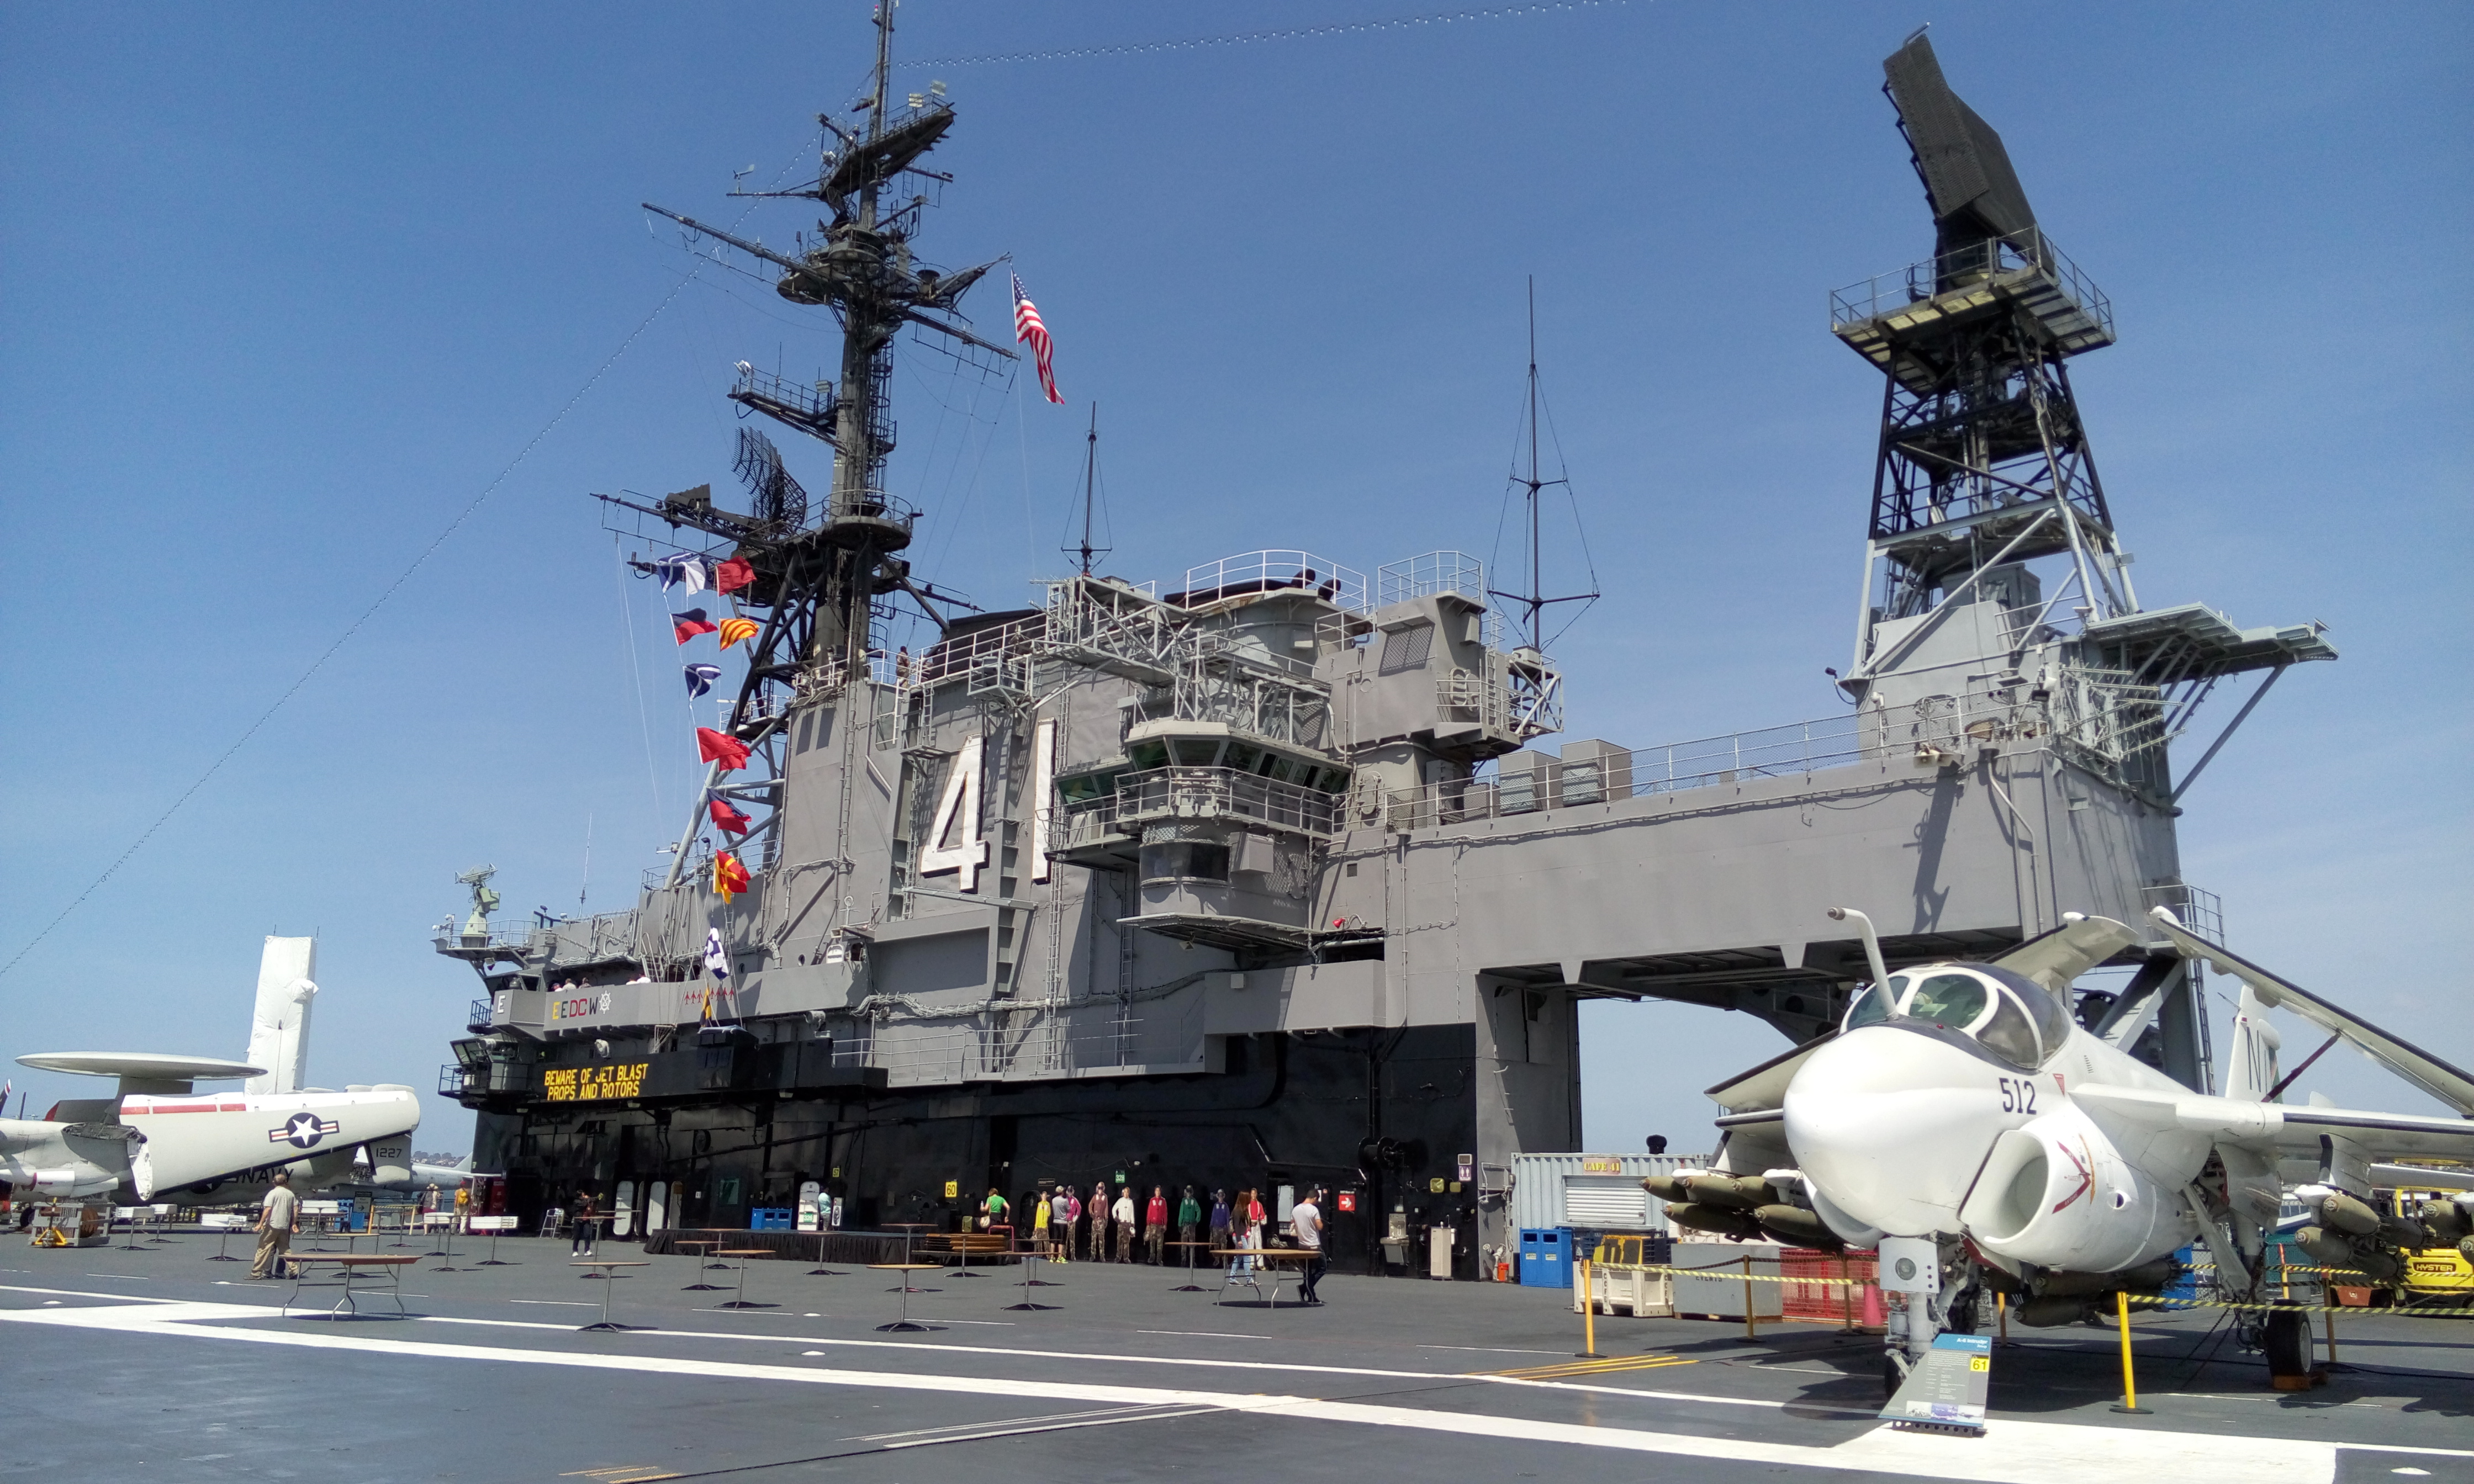
\includegraphics[width=\paperwidth,height=.4\paperheight]{15/image20160415_114740885.jpg};%
};
%\node[inner sep=0pt, yshift=.25\paperheight] at (current page.south) {%
%	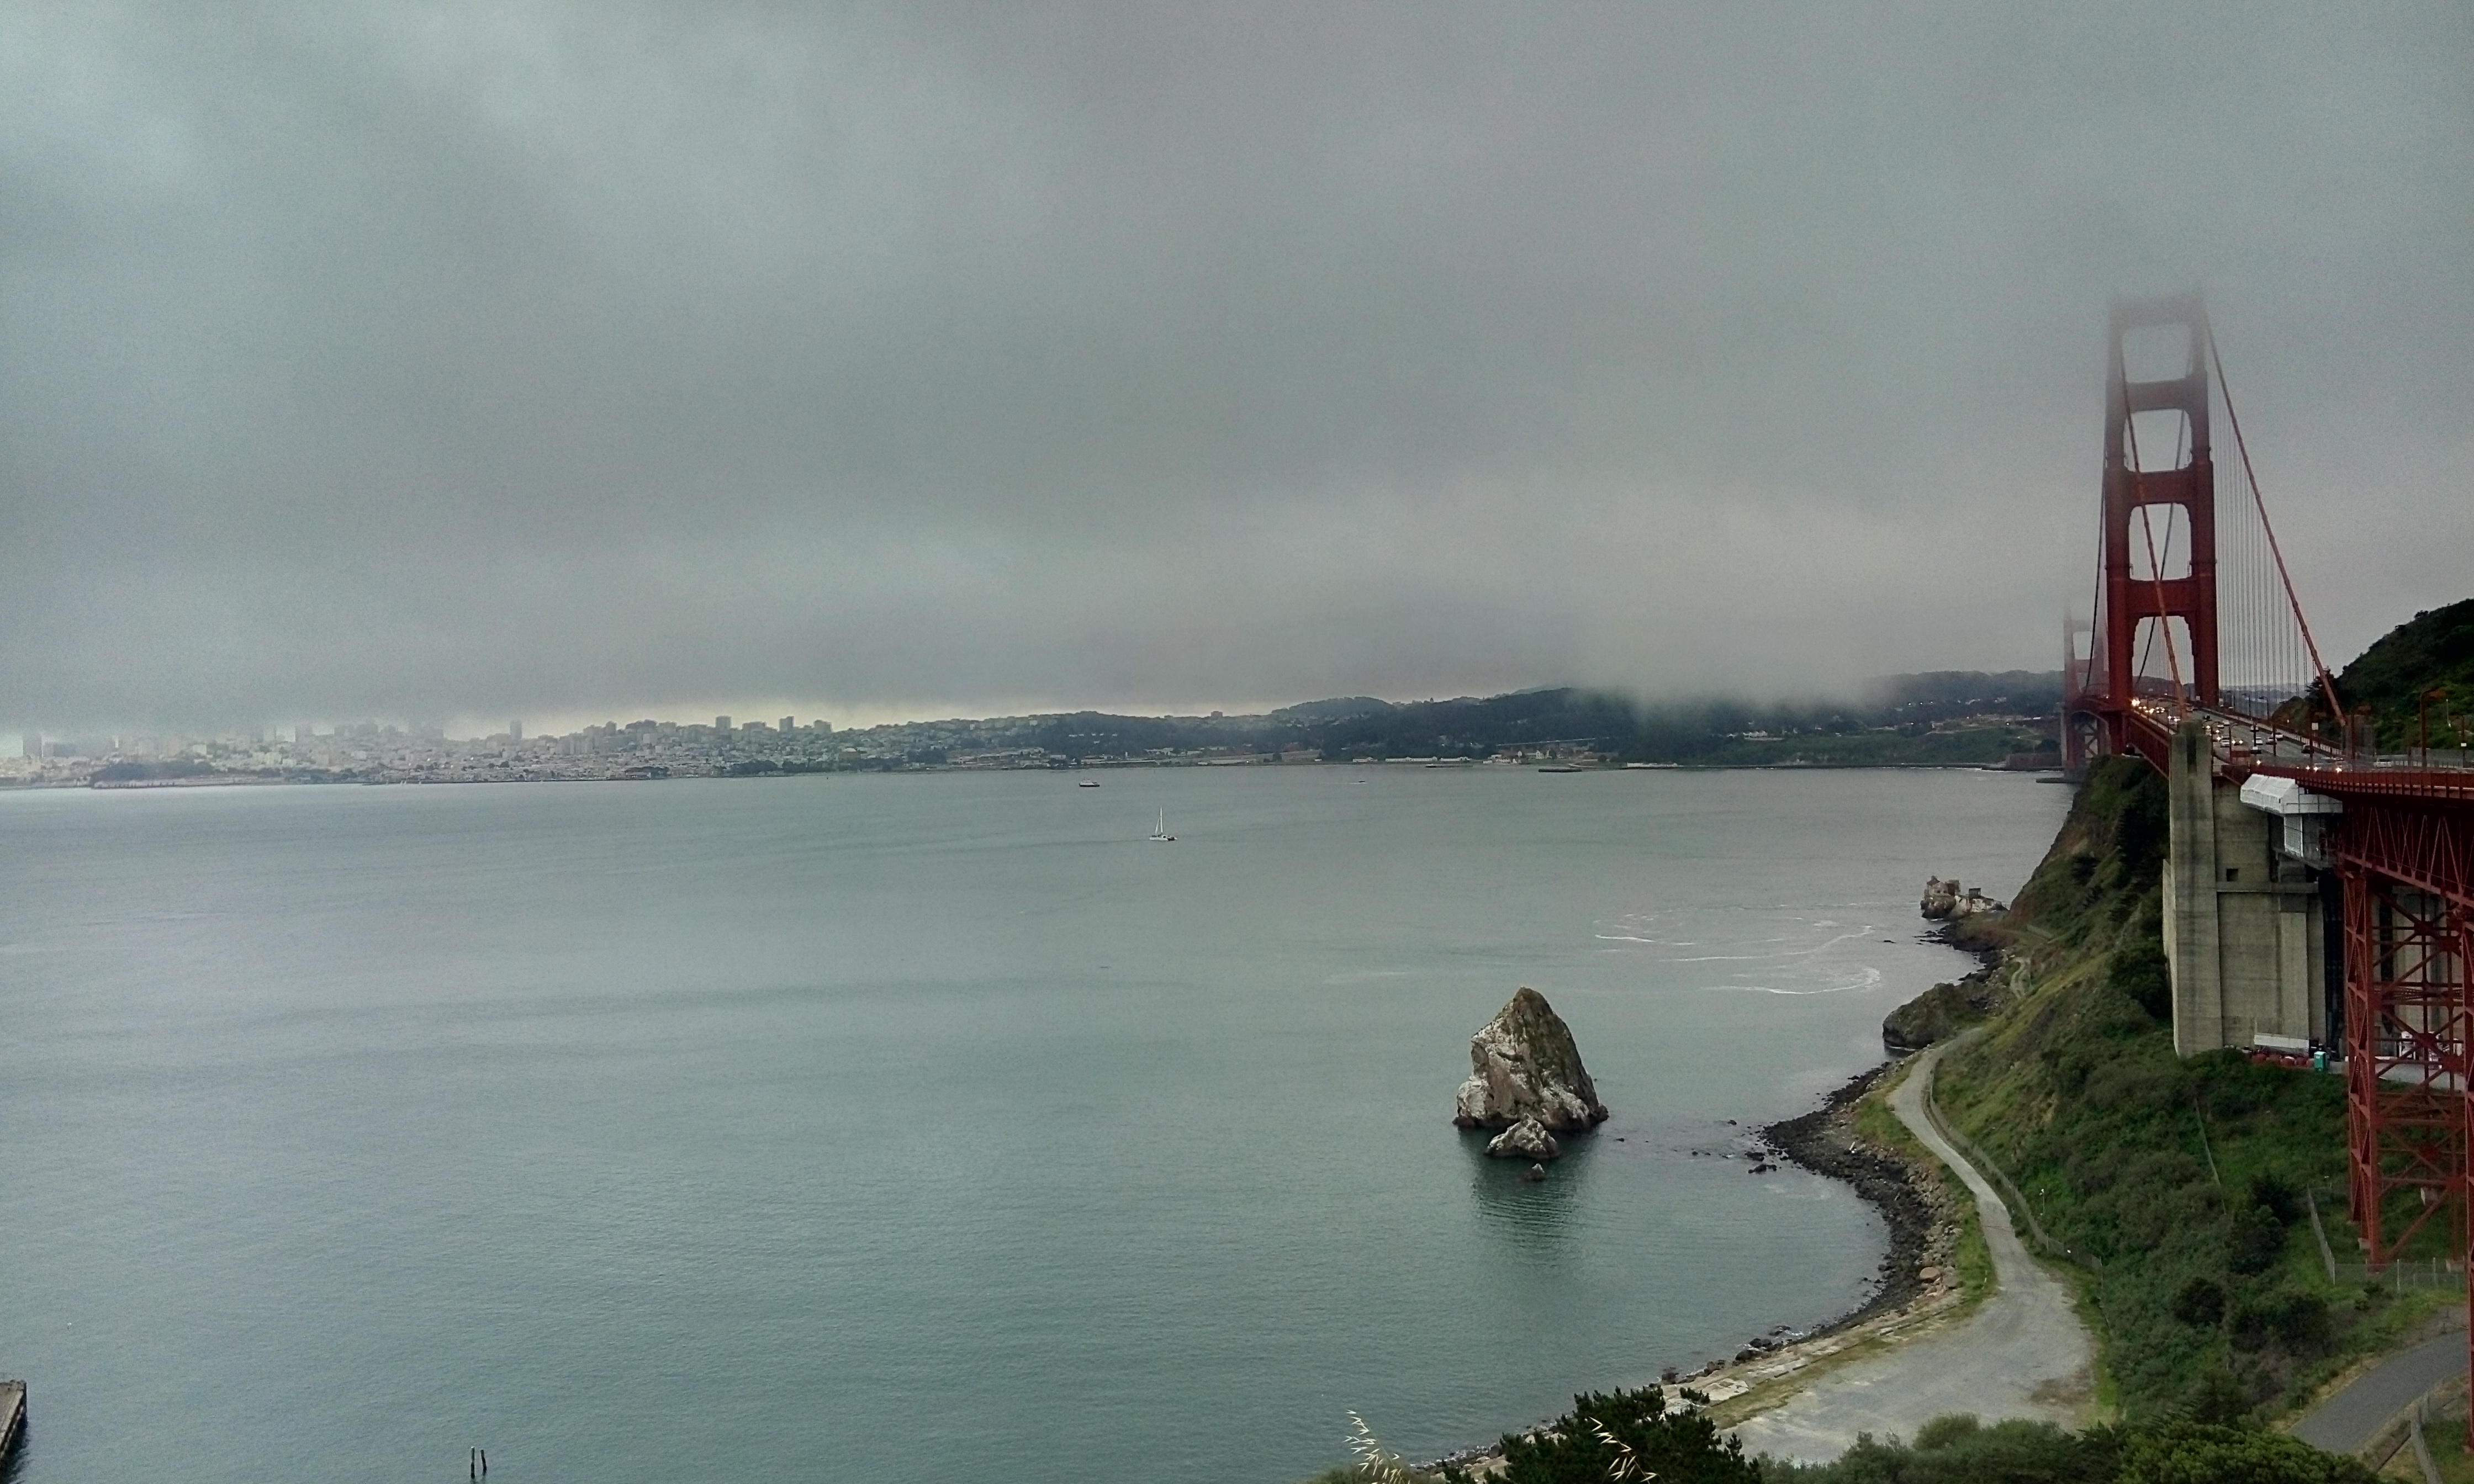
\includegraphics[width=\paperwidth,height=.5\paperheight]{21/image20160420_193101911.jpg};%
%};
\end{tikzpicture}

\vspace*{.3\paperheight}

\noindent
Deck gab es auch ein paar spaßig wirkende Flugsimulatoren, für die wir leider keine Zeit hatten.
Erst recht nicht für den Maschinenraum.

Die Parkuhr war bei unserer Rückkehr gut abgelaufen und dann ging es auch schon weiter in Richtung \TOWN{Los Angeles}.
Auf den \FOREIGN{Interstates}\footnote{Autobahn} hätte die Fahrt rund $2 \frac{1}{2}$ Stunden gedauert.
Über die gewählte \glqq historische\grqq \, \FOREIGN{Route 101} erreichten wir nach nur 6~Stunden unser Ziel.
Wir zogen die langsame Strecke der schnelleren vor in der Hoffnung so nicht wieder auf einer achtspurigen Straße zu landen.
Das war dann auch der Fall, mehr wie vier Spuren mussten wir nicht meistern.
Außerdem kamen wir so an Walen vorbei.

Für die kommenden Nächte ging es wieder ins Hostel.
Gebucht hatten wir ein 10er Zimmer, ein 8er bekamen wir und das war jede Nacht komplett belegt.
Trotz fluktuierender Kundschaft.
Mit den Übernachtungen im Hostel hatten wir gegenüber einem Hotel deutlich gespart und dann parkten wir das Auto noch für 5~\$ pro Tag statt 14~\$.
Deshalb ging es zum gehobenen Italiener.
Die Lasagne war ganz gut, die halbe Portion vom Christian ein Witz.
